\documentclass[border=5pt, multi, tikz]{standalone}
\usepackage{import}
\usepackage{amsmath}
\usepackage{amssymb}
\usetikzlibrary{positioning, arrows.meta, shapes.geometric, calc, fit, backgrounds}

% 定义颜色
\definecolor{deepcolor}{RGB}{220, 20, 60}         % 红色 - Deep (LSTM)
\definecolor{widecolor}{RGB}{255, 140, 0}         % 橙色 - Wide (Linear)
\definecolor{fusioncolor}{RGB}{70, 130, 180}      % 钢蓝 - Fusion
\definecolor{inputcolor}{RGB}{100, 149, 237}      % 浅蓝 - Input
\definecolor{outputcolor}{RGB}{60, 179, 113}      % 绿色 - Output

\begin{document}
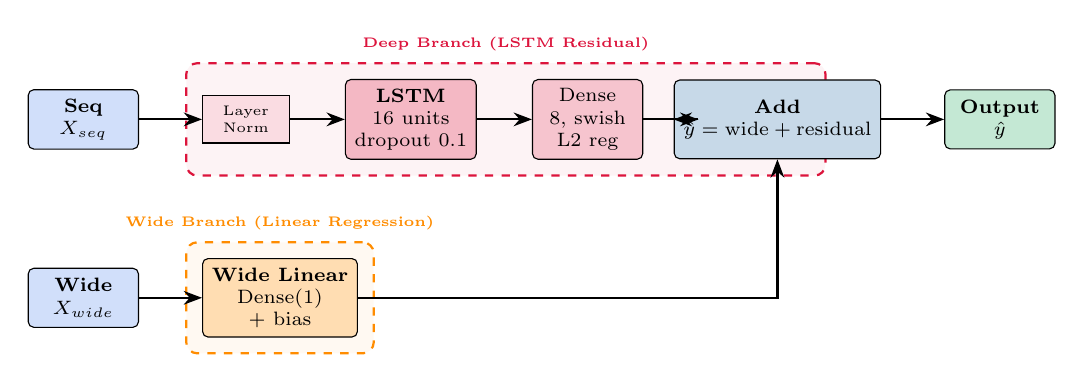
\begin{tikzpicture}[
    node distance=0.4cm and 0.7cm,
    box/.style={rectangle, draw, minimum width=1.4cm, minimum height=0.75cm, align=center, font=\scriptsize, rounded corners=2pt},
    smallbox/.style={rectangle, draw, minimum width=1.1cm, minimum height=0.6cm, align=center, font=\tiny},
    arrow/.style={-Stealth, thick},
]

% ============ 输入层 (左侧) ============
\node[box, fill=inputcolor!30] (input_seq) {\textbf{Seq}\\$X_{seq}$};
\node[box, fill=inputcolor!30, below=1.5cm of input_seq] (input_wide) {\textbf{Wide}\\$X_{wide}$};

% ============ Deep分支 (上层,LSTM残差) ============
\node[smallbox, fill=deepcolor!15, right=0.8cm of input_seq] (layernorm) {Layer\\Norm};
\node[box, fill=deepcolor!30, right=of layernorm] (lstm) {\textbf{LSTM}\\16 units\\dropout 0.1};
\node[box, fill=deepcolor!25, right=of lstm] (dense8) {Dense\\8, swish\\L2 reg};
\node[box, fill=deepcolor!40, right=of dense8] (residual) {Residual\\Dense(1)};

% ============ Wide分支 (下层,线性) ============
\node[box, fill=widecolor!30, right=0.8cm of input_wide] (wide_linear) {\textbf{Wide Linear}\\Dense(1)\\+ bias};

% ============ 融合层 (右侧) ============
\node[box, fill=fusioncolor!30, right=2.5cm of lstm, minimum height=1cm] (add) {\textbf{Add}\\$\hat{y} = \text{wide} + \text{residual}$};

% ============ 输出 ============
\node[box, fill=outputcolor!30, right=0.8cm of add] (output) {\textbf{Output}\\$\hat{y}$};

% ============ 箭头 ============
% Deep分支流程
\draw[arrow] (input_seq) -- (layernorm);
\draw[arrow] (layernorm) -- (lstm);
\draw[arrow] (lstm) -- (dense8);
\draw[arrow] (dense8) -- (residual);

% Wide分支流程
\draw[arrow] (input_wide) -- (wide_linear);

% 融合
\draw[arrow] (residual) -- (add);
\draw[arrow] (wide_linear) -| (add);

% 输出
\draw[arrow] (add) -- (output);

% ============ 背景框 ============
\begin{pgfonlayer}{background}
    % Deep分支背景 (LSTM残差路径)
    \node[draw=deepcolor, thick, dashed, rounded corners, 
          fit={(layernorm) (lstm) (dense8) (residual)}, 
          fill=deepcolor!5, inner sep=0.2cm] (deep_box) {};
    \node[above=0.02cm of deep_box, font=\tiny\bfseries, text=deepcolor] {Deep Branch (LSTM Residual)};
    
    % Wide分支背景 (线性回归)
    \node[draw=widecolor, thick, dashed, rounded corners, 
          fit={(wide_linear)}, 
          fill=widecolor!5, inner sep=0.2cm] (wide_box) {};
    \node[above=0.02cm of wide_box, font=\tiny\bfseries, text=widecolor] {Wide Branch (Linear Regression)};
\end{pgfonlayer}

\end{tikzpicture}
\end{document}
